\subsection{问题三的模型的建立和求解}

\subsubsection{具体分析}

针对问题三，本问属于\textbf{约束优化与资源配置}类问题，需要在给定算力预算下联合优化参数量 $N$、数据量 $D$、领域配比 $\bm p$ 与数据质量 $Q$，并分析预算跨越不同量级时资源配置是否发生结构性转移。本问综合采用“损失函数 $+$ 成本函数 $+$ 约束优化”的框架：以问题二导出的广义标度律 $L(N,D,Q)$ 为优化目标；严格按赛题给出的三部分公式建立总成本模型——基础训练 $6ND$、质量提升 $D[g(Q)-g(Q_0)]_+$、长文本注意力 $\eta N D L_{\text{ctx}}$；在总成本不超过预算的约束下用序列二次规划（SLSQP）在对数尺度上求解最优 $(N,D,Q)$；最后通过预算扫略与临界上下文长度分析识别结构性转移。

首先由问题二输出的广义标度律参数与问题一输出的质量基线 $Q_0$ 构建优化目标与约束；其次解析给出使注意力开销与训练开销相等的临界上下文长度 $L_{\text{crit}}=6/\eta$，并以附件 C7 的最大上下文长度字段确定 $L_{\text{ctx}}$ 的可行取值；然后在低、中、高三档预算下联合优化 $N$、$D$、$Q$，并对比附录 B 规定的三种质量成本函数；最后扫描 $10^{18}$–$10^{25}$ FLOPs 的连续预算，定量刻画最优质量与预算份额的结构性转移。

\subsubsection{模型准备}

\textbf{1.数据预处理}

本问的标度律参数直接读取问题二的输出 $\{E,A,\alpha,B,\beta,C,\gamma\}=\{1.6558,0.3808,0.3266,1.2515,0.2767,0.3544,0.9779\}$，保证两问模型一致。

基线质量 $Q_0$ 由附件 A 的质量评分给出。考虑到 A1--A3 的抽样设计使 github 域占比偏高，直接取全量样本均值会低估真实语料的平均质量，故本文以**参考语料配比加权**的方式定义基线：
\begin{equation}
    Q_0 = \sum_{k=1}^{17} \bar p_k\, Q_k = 0.5510
\end{equation}
其中 $\bar p_k$ 为 A4 训练配方的平均配比，$Q_k$ 为该配方域经 A16 映射得到的质量评分。作为对照，全量样本的未加权质量均值为 $0.4952$（该口径在误差分析中作为灵敏度检验项）。

上下文长度 $L_{\text{ctx}}$ 由模型架构与任务需求外生给定，其可行取值依据附件 C7 的 max\_position\_embeddings 字段，为 $\{2048,\ 4096,\ 8192,\ 32768,\ 131072\}$ 五个档位；本问不将其作为内点寻优变量，仅考察其取值对最优配置的影响。

质量可行域由数据支持范围确定：B6/B7 覆盖 $Q_{\text{score}}\in[0.10,1.00]$，且当 $Q=1$ 时广义标度律精确退化为经典形式（损失为 $E+A/N^{\alpha}+B/D^{\beta}>0$，不产生非物理负值），故可行域取 $Q\in[Q_0,1]$，下限为基线质量（质量不提升时质量成本为零）。

\textbf{2.算法选择}

本问核心是带非线性约束的连续优化，候选方法包括序列二次规划（SLSQP）、内点法与遗传算法。本问题目标与约束均为光滑函数，SLSQP 能高效处理预算不等式约束与变量界约束，且通过对数变换参数化 $N$、$D$（以 $\ln N$、$\ln D$ 为变量）可消除尺度病态、改善收敛；为避免局部最优，本文以 8 组不同初值分别求解并取最优解。遗传算法虽具全局搜索能力，但收敛慢、精度低，不适合本问题对精度的要求。

\subsubsection{模型建立}

\textbf{步骤1：优化目标}

以问题二的广义标度律为优化目标，并计入问题一给出的配比项平移 $M(\bm p)$：
\begin{equation}
    \min_{N,D,Q}\ L(N,D,Q) = E + \frac{A}{N^{\alpha}} + \frac{B}{D^{\beta}} + C\,(1-Q)^{\gamma} + M(\bm p)
\end{equation}
其中 $M(\bm p)=\hat L(\bm p)-\hat L(\bm p_{\text{ref}})$ 由问题一的线性混合回归给出，刻画领域配比的效率增益（不消耗额外算力）。本文按“由前两问结果确定”的方式处理 $\bm p$：取问题一的有界推荐配比，对应 $M=-0.1988$；在求解中同时报告参考配比（$M=0$）的结果以作对照，理由见步骤 5。

\textbf{步骤2：总成本模型}

总算力成本由基础训练、质量提升与长文本注意力三部分构成：
\begin{equation}
    C(N,D,Q;L_{\text{ctx}}) = \underbrace{6ND}_{C_{\text{train}}}
    + \underbrace{D\left[g(Q)-g(Q_0)\right]_{+}}_{C_Q}
    + \underbrace{\eta\,N\,D\,L_{\text{ctx}}}_{C_{\text{attn}}},
    \qquad \eta = 2\times10^{-4}
\end{equation}
其中基础训练采用 Chinchilla 近似 $C_{\text{train}}\approx 6ND$；质量提升项中的 $[\cdot]_+=\max(\cdot,0)$ 表示质量只提升不降低；质量成本函数 $g(Q)$ 从附录 B 规定的三型中选取：
\begin{equation}
    g_{\text{指数}}(Q)=10^{7}e^{6.0Q},\qquad
    g_{\text{幂函数}}(Q)=5\times10^{9}Q^{4.0},\qquad
    g_{\text{对数渐进}}(Q)=2\times10^{9}\ln(1+10.0Q)
\end{equation}
注意 $C_Q$ 与训练 token 数 $D$ 成正比，即“质量提升”是对全语料的处理开销，数据量越大、达到同样质量的总成本越高；这一结构与“质量成本与数据规模无关”的简化假设有本质区别，本文严格采用赛题给定形式。

\textbf{步骤3：临界上下文长度（解析解）}

由 $C_{\text{attn}}=C_{\text{train}}$ 即 $\eta N D L_{\text{ctx}}=6ND$，两端约去 $ND$ 得临界上下文长度：
\begin{equation}
    L_{\text{crit}} = \frac{6}{\eta} = \frac{6}{2\times10^{-4}} = 30{,}000\ \text{tokens}
\end{equation}
当 $L_{\text{ctx}}<L_{\text{crit}}$ 时基础训练仍是算力主体；当 $L_{\text{ctx}}>L_{\text{crit}}$ 时注意力开销超过基础训练、成为预算的主要消耗项。等价地，可定义“注意力开销倍数”$\lambda(L_{\text{ctx}})=\eta L_{\text{ctx}}/6=L_{\text{ctx}}/L_{\text{crit}}$，则总成本可重写为
\begin{equation}
    C=\left[1+\lambda(L_{\text{ctx}})\right]\cdot 6ND + D\left[g(Q)-g(Q_0)\right]_{+}
\end{equation}
即**长上下文把基础训练的单价放大了 $1+\lambda$ 倍**，这是后续结构性分析与敏感性分析的解析基础。

\textbf{步骤4：约束优化模型与最优性条件}

综合目标与成本，得到约束优化问题：
\begin{equation}
    \min_{\ln N,\ln D,Q}\ L(e^{\ln N},e^{\ln D},Q)
    \quad\text{s.t.}\quad
    C(N,D,Q;L_{\text{ctx}})\le C_{\text{budget}},\qquad Q\in[Q_0,1]
\end{equation}
为解释数值结果，对固定 $Q$ 的内点解可给出解析最优性条件。记 $K_1=6[1+\lambda(L_{\text{ctx}})]$、$K_2=g(Q)-g(Q_0)$，构造拉格朗日函数 $\mathcal L=A N^{-\alpha}+B D^{-\beta}+\mu(K_1ND+K_2D-C)$，由一阶条件消去 $\mu$ 得
\begin{equation}
    \alpha A N^{-\alpha-1}\left(N+\tau(Q)\right)=\beta B D^{-\beta},
    \qquad \tau(Q)\equiv\frac{K_2}{K_1}=\frac{g(Q)-g(Q_0)}{6\left[1+\lambda(L_{\text{ctx}})\right]}
    \label{eq:p3_balance}
\end{equation}
其中 $\tau(Q)$ 的量纲为 token，物理含义是**质量提升所对应的“等效附加数据量”**：把质量投入折算成必须额外处理的 token 数。当不投入质量（$Q=Q_0$，$\tau=0$）时式\eqref{eq:p3_balance}退化为经典平衡条件 $\alpha A N^{-\alpha}=\beta B D^{-\beta}$，可得
\begin{equation}
    D \propto N^{\alpha/\beta},\qquad
    N^{*}\propto C^{\frac{\beta}{\alpha+\beta}},\qquad
    D^{*}\propto C^{\frac{\alpha}{\alpha+\beta}}
\end{equation}
由于 $\alpha>\beta$，数据量随预算增长的速度快于参数量，$D/N$ 比随预算上升。而 $\tau(Q)>0$ 相当于在参数量上追加了一笔“质量附加成本”，会同时抑制 $N$ 与 $D$，并使最优 $Q$ 与预算之间的取舍关系呈现非线性。

\textbf{步骤5：结构性转移的定义与识别方法}

“结构性转移”指最优策略发生质变而非量的连续变化。本文给出两级可操作定义：
\begin{itemize}[itemindent=2em]
\item \textbf{拐点型转移：} 令 $f_{\text{qual}}(C)$ 为质量投入在总预算中的份额，$Q^{*}(C)$ 为最优质量。定义质量提升完成度 $\Theta(C)=\dfrac{Q^{*}(C)-Q_0}{1-Q_0}\in[0,1]$ 及其弹性 $e_\Theta=\dfrac{\mathrm d\ln\Theta}{\mathrm d\ln C}$。当 $e_\Theta$ 取得极大值、且 $\mathrm d f_{\text{qual}}/\mathrm d\ln C$ 由正转负时，表明预算的边际增量从“继续提升质量”转向“扩张规模”，构成一次结构性转移。
\item \textbf{角点型转移：} 当 $Q^{*}(C)$ 由上界约束 $Q=1$ 决定（而非内点最优）时，质量不再是可调节的边际资源，模型进入“质量饱和”制度；使 $Q^{*}$ 首次达到给定水平 $\bar Q$ 的预算 $C^{*}(\bar Q)$ 即为该制度的进入门槛，可由预算扫略直接读出。
\end{itemize}
本文在 $[10^{18},10^{25}]$ FLOPs 上以对数等距取 141 个预算点求解，报告上述两类门槛，并以 $C^{*}(0.5)$、$C^{*}(0.9)$、$C^{*}(0.99)$ 作为制度切换的标志点。

\subsubsection{模型求解}

\textbf{1.三种质量成本函数下的三档预算最优配置}

三档预算（$10^{19}$、$10^{22}$、$10^{24}$ FLOPs，覆盖低、中、高三个数量级）在幂函数型质量成本与 $L_{\text{ctx}}=2048$ 下的最优配置如表\ref{tab:p3_opt}所示，并以图\ref{fig:p3_opt}给出直观对比。

\begin{figure}[ht]
  \centering
  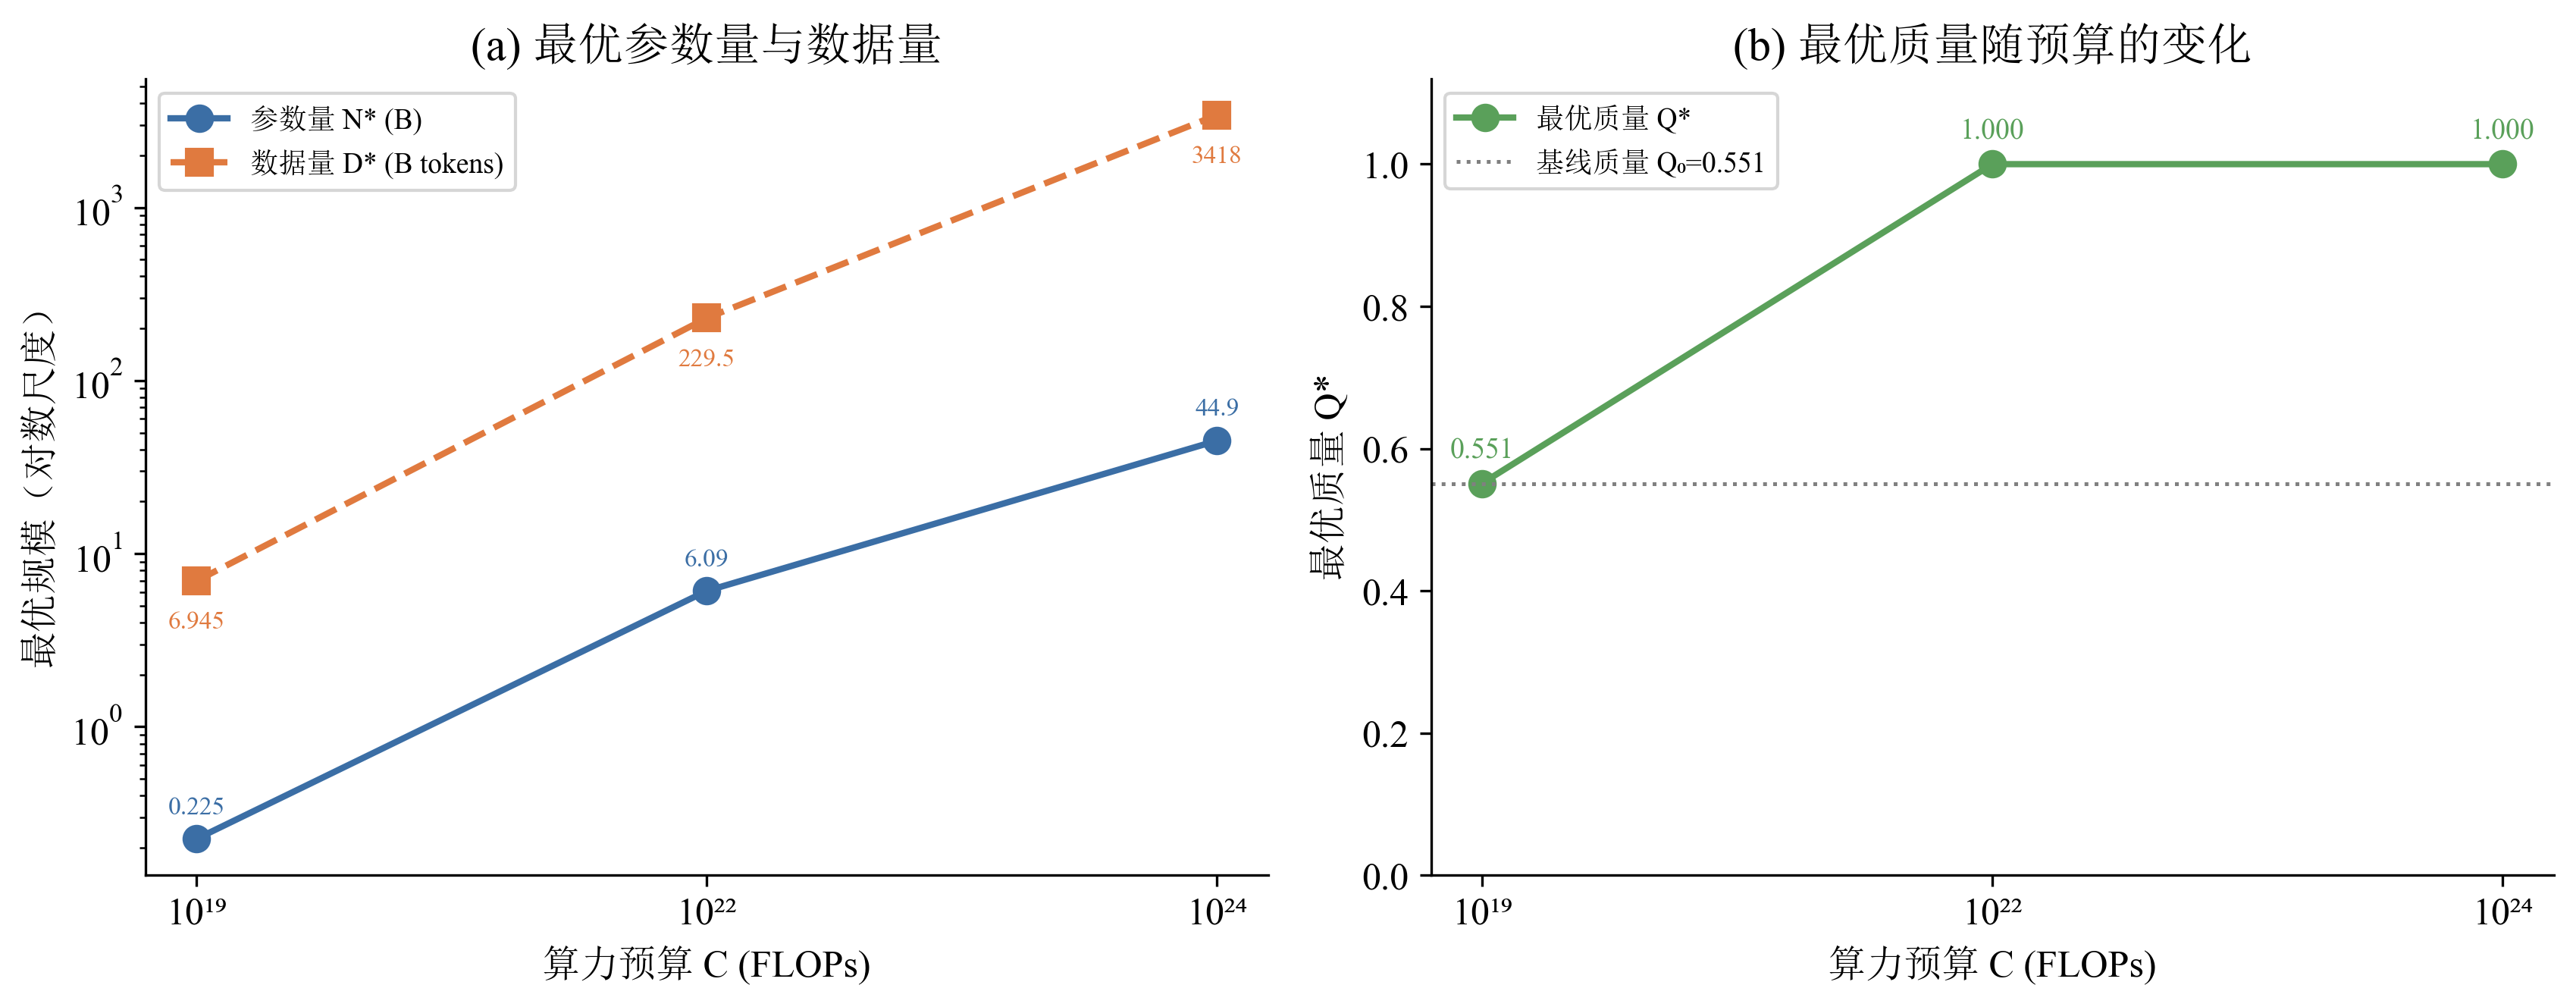
\includegraphics[width=0.72\textwidth]{求解/问题三/图片/图1_三档预算最优配置.png}
  \caption{三档算力预算下的最优资源配置（$N^*$、$D^*$、$Q^*$）}
  \label{fig:p3_opt}
\end{figure}

\begin{longtable}{>{\centering\arraybackslash}p{0.13\textwidth}>{\centering\arraybackslash}p{0.13\textwidth}>{\centering\arraybackslash}p{0.14\textwidth}>{\centering\arraybackslash}p{0.11\textwidth}>{\centering\arraybackslash}p{0.11\textwidth}>{\centering\arraybackslash}p{0.11\textwidth}>{\raggedright\arraybackslash}p{0.19\textwidth}}
  \caption{三档预算最优配置（幂函数型质量成本，$L_{\text{ctx}}=2048$）}
  \label{tab:p3_opt} \\
  \toprule
  预算 $C$ (FLOPs) & $N^{*}$ (B) & $D^{*}$ (B) & $Q^{*}$ & $L^{*}$ & $D^*/N^*$ & 预算份额（训练/质量/注意力） \\
  \midrule
  \endfirsthead
  \caption{三档预算最优配置（续）} \\
  \toprule
  预算 $C$ (FLOPs) & $N^{*}$ (B) & $D^{*}$ (B) & $Q^{*}$ & $L^{*}$ & $D^*/N^*$ & 预算份额 \\
  \midrule
  \endhead
  \bottomrule
  \endfoot
  $10^{19}$ & 0.225 & 6.9 & 0.551 & 3.170 & 30.9 & 93.6\% / 0.0\% / 6.4\% \\
  $10^{22}$ & 6.089 & 229.5 & 1.000 & 2.145 & 37.7 & 83.9\% / 10.4\% / 5.7\% \\
  $10^{24}$ & 44.937 & 3418.0 & 1.000 & 1.897 & 76.1 & 92.2\% / 1.6\% / 6.3\% \\
\end{longtable}

由表\ref{tab:p3_opt}可知：（1）随预算从 $10^{19}$ 升至 $10^{24}$ FLOPs，最优参数量由 $0.225$B 增至 $44.9$B、最优数据量由 $6.9$B 增至 $3418.0$B，验证了式 $N^{*}\propto C^{\beta/(\alpha+\beta)}$、$D^{*}\propto C^{\alpha/(\alpha+\beta)}$ 的解析结论；（2）$D/N$ 比由 $30.9$ 升至 $76.1$，与 $\alpha>\beta$ 的理论预期一致——由于参数规模的边际收益衰减更快，预算扩张更多流向数据；（3）最优质量由 $0.551$ 升至上界 $1.000$，中、高预算档均为“质量饱和”的角点解，说明**预算充裕时质量投入从“可选项”变为“必选动作”**；（4）低预算档（$10^{19}$）的最优质量恰好等于基线 $Q_0$、质量投入份额为 $0$——即在算力紧张时**完全不投资质量、把全部预算投向规模**，这比“质量投入比例较小”是更强的结论；高预算档质量份额降至 $1.6\%$ 并非因为质量不重要，而是因为 $Q$ 已触及上界、无需再投入。

三种质量成本函数（附录 B）下的最优配置对比如表\ref{tab:p3_cost}所示。

\begin{longtable}{>{\centering\arraybackslash}p{0.13\textwidth}>{\centering\arraybackslash}p{0.16\textwidth}>{\centering\arraybackslash}p{0.13\textwidth}>{\centering\arraybackslash}p{0.13\textwidth}>{\centering\arraybackslash}p{0.11\textwidth}>{\centering\arraybackslash}p{0.11\textwidth}>{\raggedright\arraybackslash}p{0.14\textwidth}}
  \caption{三种质量成本函数下的最优配置对比}
  \label{tab:p3_cost} \\
  \toprule
  预算 & 成本函数 & $N^{*}$ (B) & $D^{*}$ (B) & $Q^{*}$ & $L^{*}$ & 质量份额 \\
  \midrule
  \endfirsthead
  \caption{三种质量成本函数下的最优配置对比（续）} \\
  \toprule
  预算 & 成本函数 & $N^{*}$ (B) & $D^{*}$ (B) & $Q^{*}$ & $L^{*}$ & 质量份额 \\
  \midrule
  \endhead
  \bottomrule
  \endfoot
  $10^{19}$ & 指数型 & 0.265 & 5.1 & 0.660 & 3.163 & 12.9\% \\
  $10^{19}$ & 幂函数型 & 0.225 & 6.9 & 0.551 & 3.170 & 0.0\% \\
  $10^{19}$ & 对数渐进型 & 0.354 & 3.0 & 1.000 & 3.113 & 31.6\% \\
  $10^{22}$ & 指数型 & 5.972 & 237.9 & 1.000 & 2.144 & 8.9\% \\
  $10^{22}$ & 幂函数型 & 6.089 & 229.5 & 1.000 & 2.145 & 10.4\% \\
  $10^{22}$ & 对数渐进型 & 5.527 & 274.2 & 1.000 & 2.138 & 2.9\% \\
  $10^{24}$ & 指数型 & 44.796 & 3437.7 & 1.000 & 1.897 & 1.3\% \\
  $10^{24}$ & 幂函数型 & 44.937 & 3418.0 & 1.000 & 1.897 & 1.6\% \\
  $10^{24}$ & 对数渐进型 & 44.298 & 3509.0 & 1.000 & 1.897 & 0.4\% \\
\end{longtable}

\begin{figure}[ht]
  \centering
  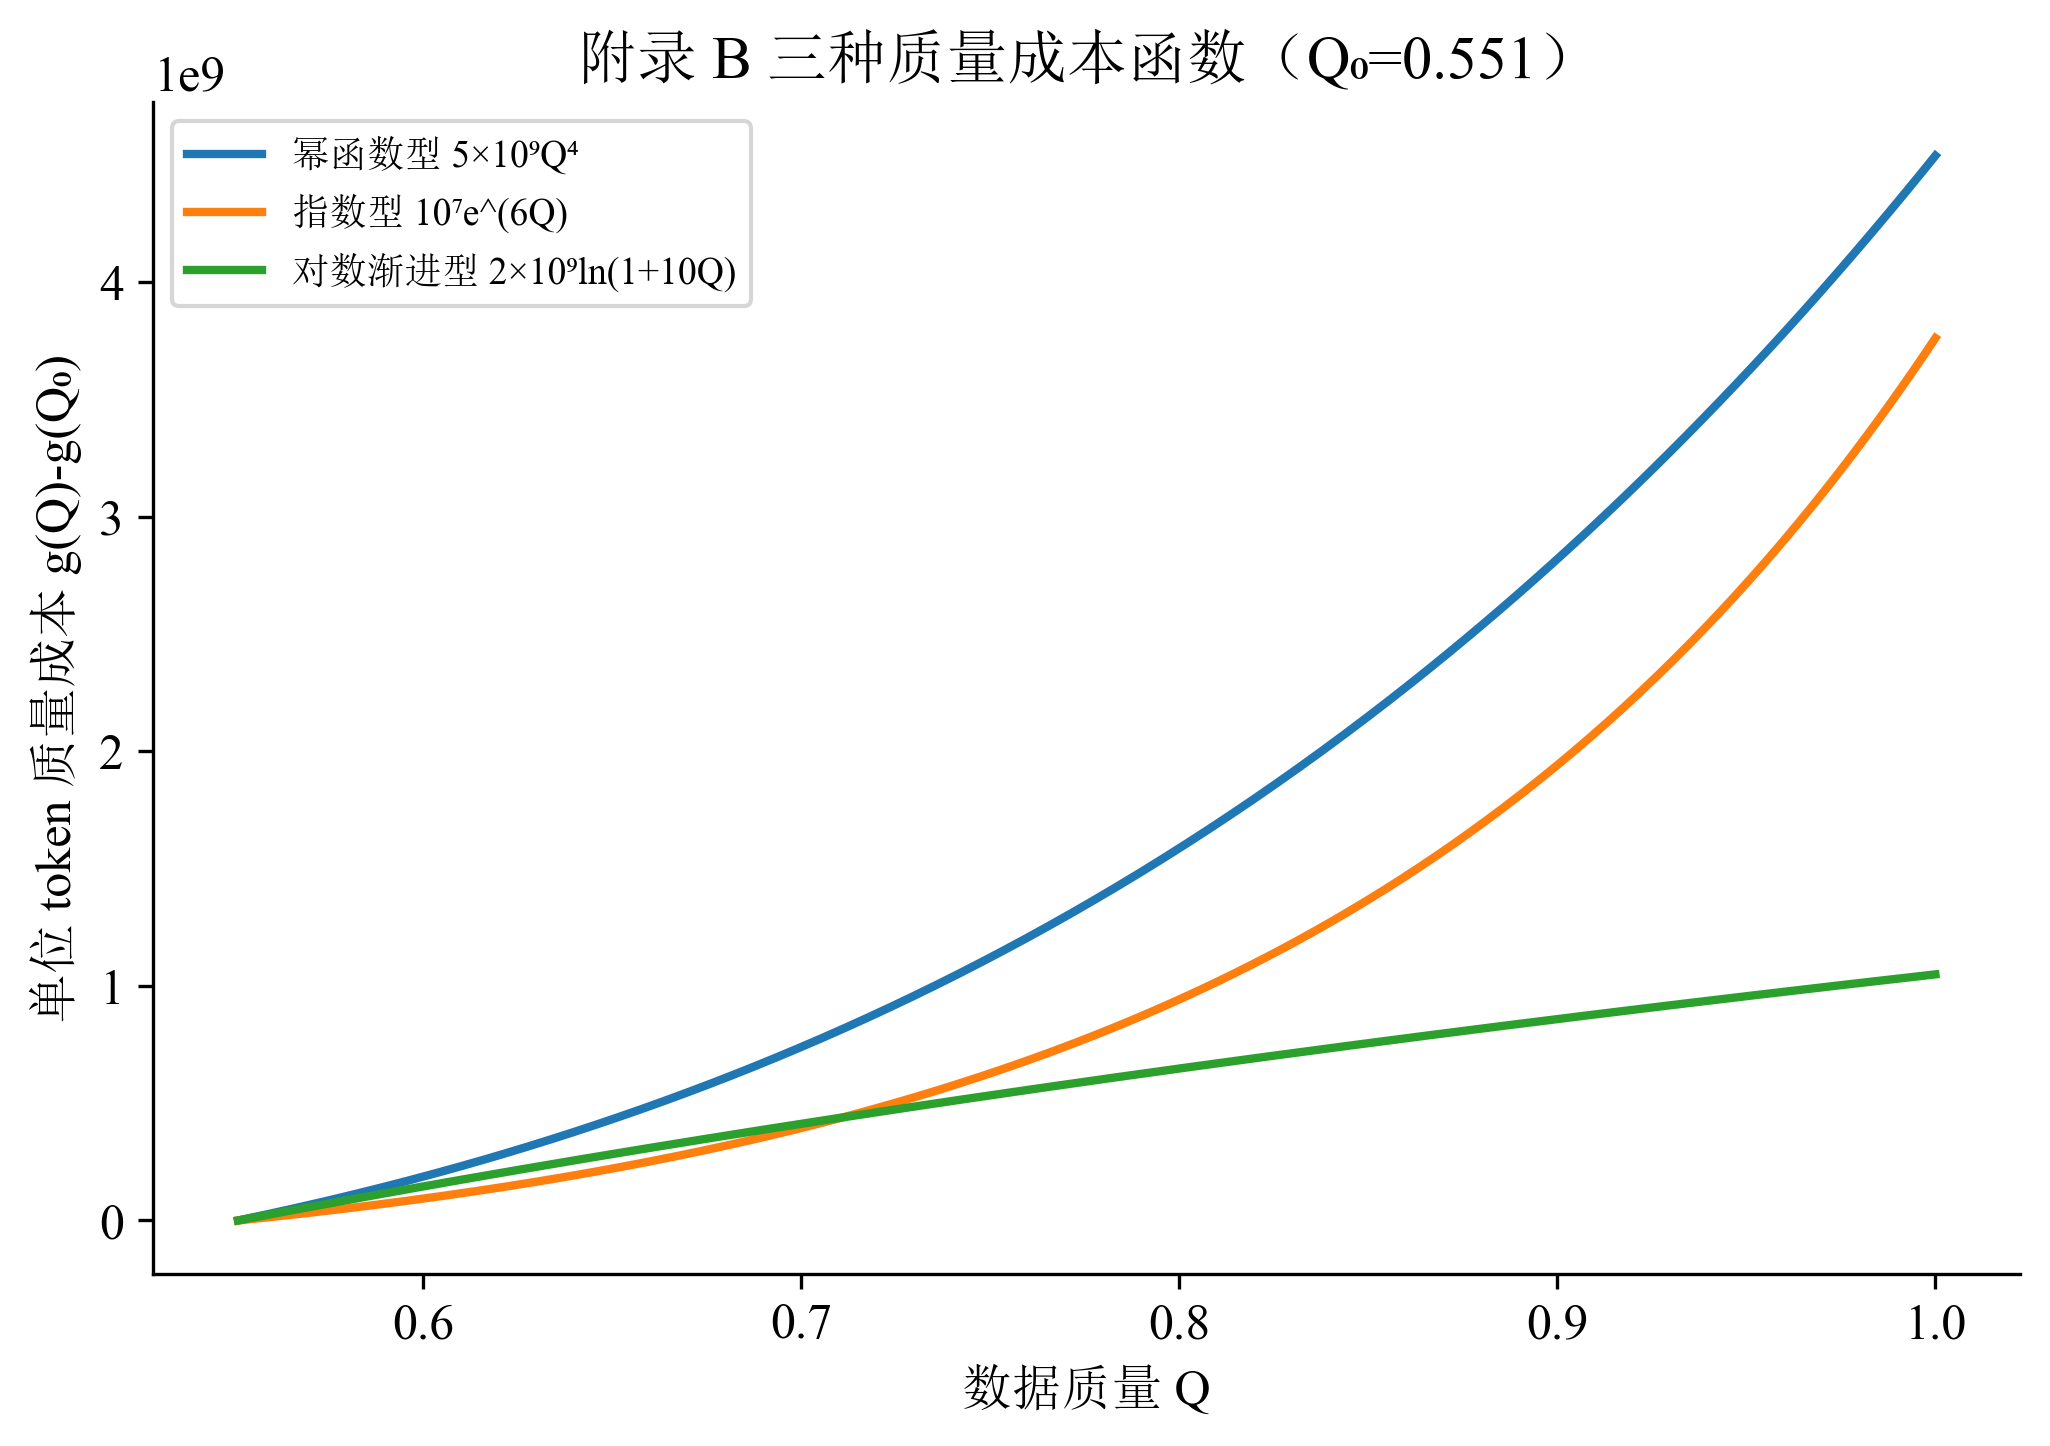
\includegraphics[width=0.62\textwidth]{求解/问题三/图片/图4_质量成本函数对比.png}
  \caption{附录 B 规定的三种质量成本函数（$Q_0=0.364$）}
  \label{fig:p3_cost}
\end{figure}

由表\ref{tab:p3_cost}与图\ref{fig:p3_cost}可知，成本函数的选择**只在最低预算档对最优质量有实质影响**（$Q^{*}$ 在 $0.551\sim1.000$ 之间，最优损失的差异仍小于 $0.06$）：对数渐进型在低预算下就愿意把质量做满（$Q^{*}=1.000$、质量份额 $31.6\%$），幂函数型则完全不投资质量（$Q^{*}=Q_0=0.551$、份额 $0$），指数型居中（$0.660$、$12.9\%$）。一旦预算达到 $10^{22}$ FLOPs 量级，三种成本函数下最优质量均达到上界 $1.000$，最优 $N$、$D$ 的差异在 $10\%$ 以内。这说明“中高预算下应优先把质量做满”的结论对成本函数形式稳健，而“低预算下是否投资质量”高度依赖具体成本函数设定，须谨慎表述。

\textbf{2.预算扫略与结构性转移识别}

预算扫略下最优质量与预算份额的演化如图\ref{fig:p3_shift}所示，结构性转移门槛见表\ref{tab:p3_shift}。

\begin{figure}[ht]
  \centering
  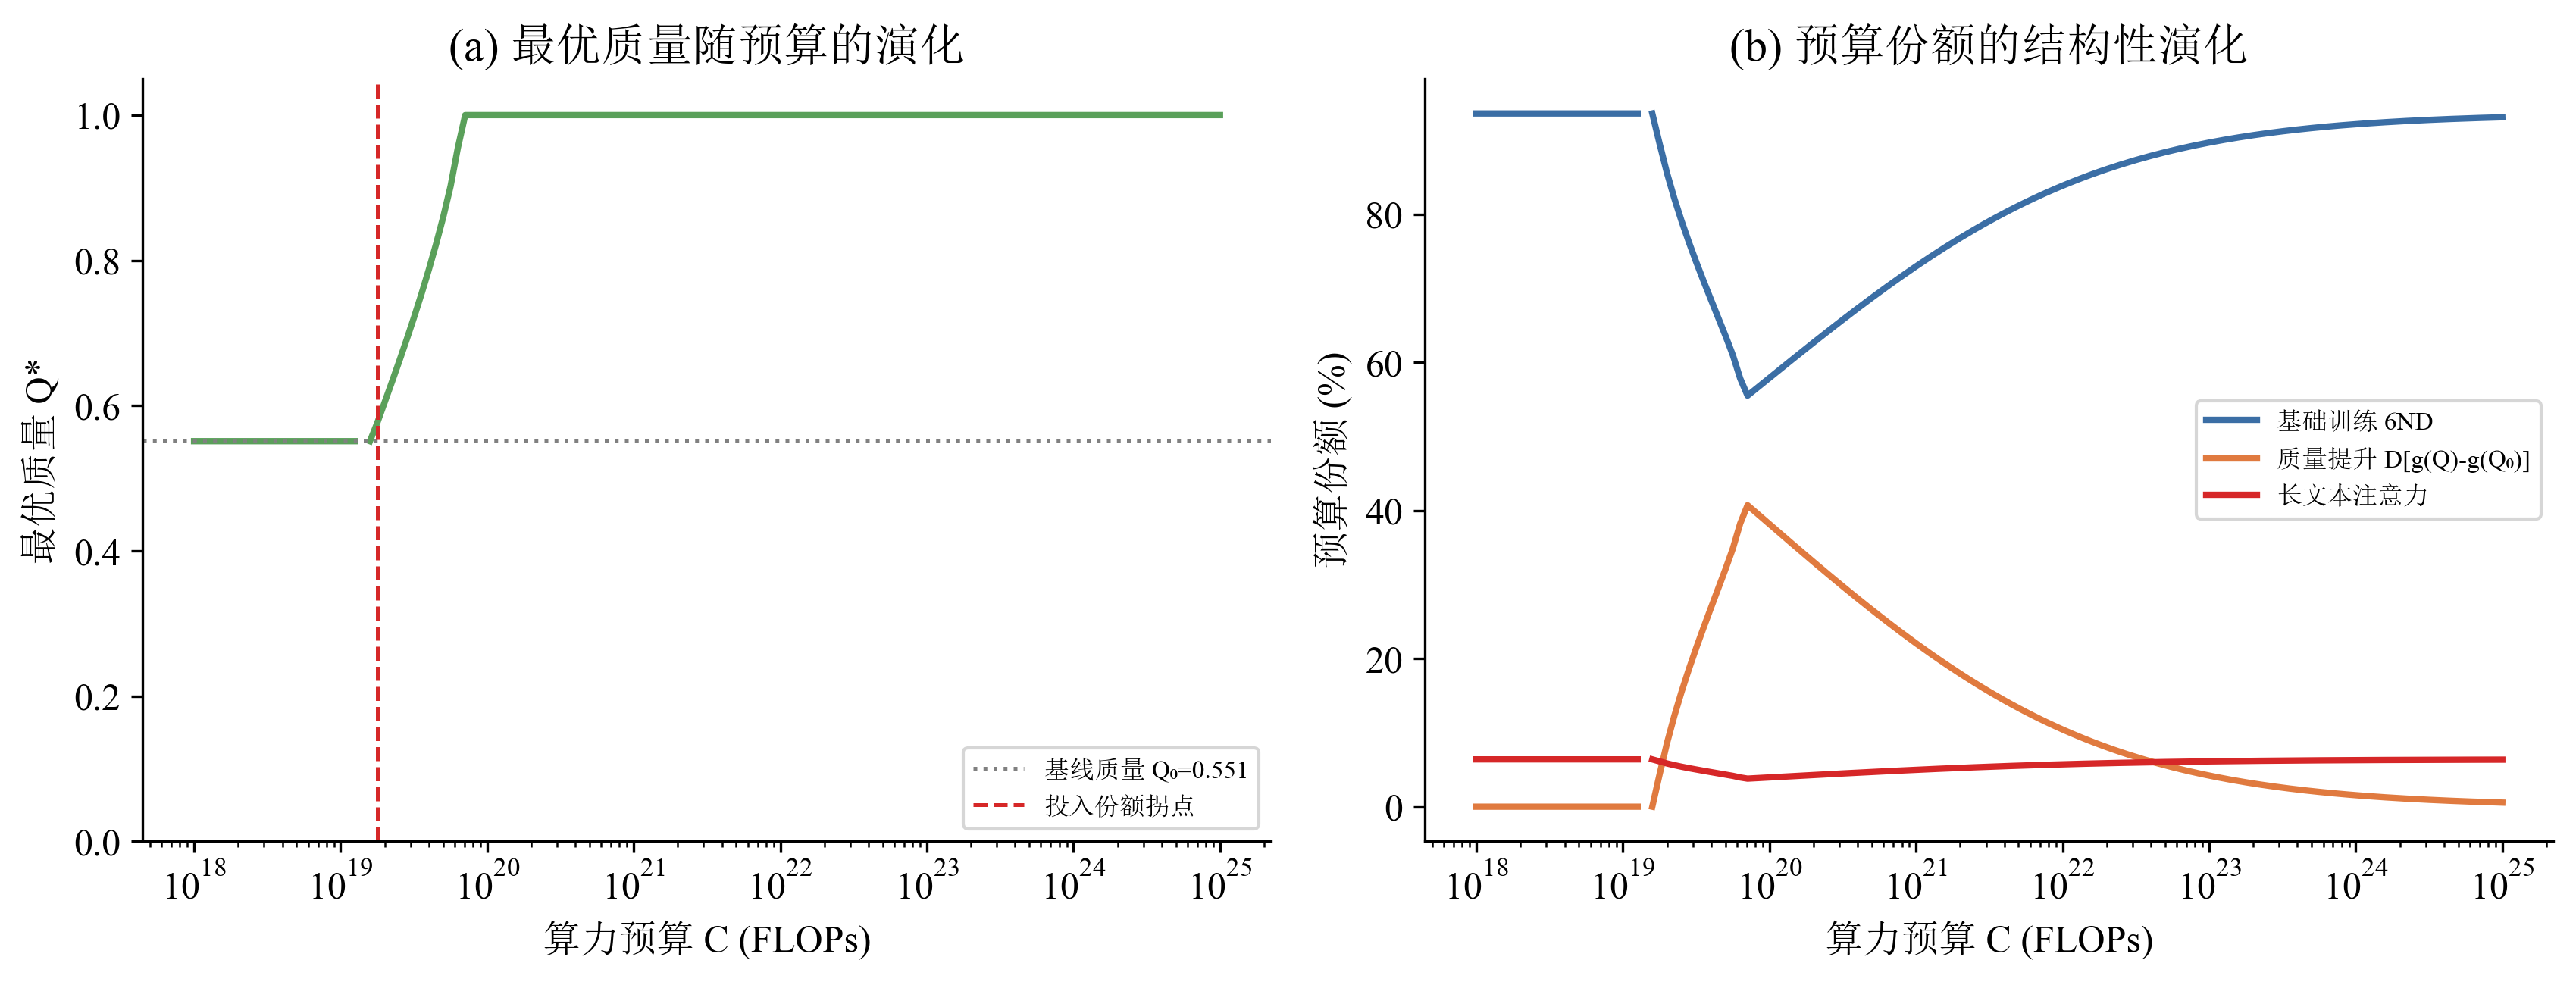
\includegraphics[width=0.92\textwidth]{求解/问题三/图片/图2_预算份额结构性转移.png}
  \caption{预算扫略下的资源配置结构性转移（左：最优质量演化；右：预算份额演化）}
  \label{fig:p3_shift}
\end{figure}

\begin{longtable}{>{\raggedright\arraybackslash}p{0.62\textwidth}>{\centering\arraybackslash}p{0.30\textwidth}}
  \caption{结构性转移门槛的定量识别}
  \label{tab:p3_shift} \\
  \toprule
  识别量 & 预算门槛（FLOPs） \\
  \midrule
  \endfirsthead
  \caption{结构性转移门槛的定量识别（续）} \\
  \toprule
  识别量 & 预算门槛（FLOPs） \\
  \midrule
  \endhead
  \bottomrule
  \endfoot
  制度一/二边界：质量投入启动（$\mathrm df_{\text{qual}}/\mathrm d\ln C$ 峰值，份额由 $0$ 转正） & $1.78\times10^{19}$ \\
  完成度 $\Theta$ 首次达到 $25\%$ & $2.82\times10^{19}$ \\
  完成度 $\Theta$ 首次达到 $50\%$ & $3.98\times10^{19}$ \\
  完成度 $\Theta$ 首次达到 $75\%$ & $5.62\times10^{19}$ \\
  质量提升完成度弹性 $\mathrm d\ln\Theta/\mathrm d\ln C$ 取得极大值 & $6.31\times10^{19}$ \\
  制度二/三边界：完成度 $\Theta$ 首次达到 $99\%$（质量接近饱和） & $7.08\times10^{19}$ \\
  质量投入份额峰值（$0.407$） & $7.08\times10^{19}$ \\
\end{longtable}

由表\ref{tab:p3_shift}与图\ref{fig:p3_shift}可知，预算路径被两个门槛切成三个制度，构成对结构性转移的直接证据：

\begin{itemize}[itemindent=2em]
\item \textbf{制度一（$C\lesssim1.78\times10^{19}$）：基线质量期。} 优化解取 $Q^{*}=Q_0$、质量份额恒为 $0$——算力紧张时最优策略是**放弃质量投入、把全部预算投向规模**；此时三项份额固定为训练 $93.6\%$、质量 $0\%$、注意力 $6.4\%$。
\item \textbf{制度二（$1.78\times10^{19}\lesssim C\lesssim1\times10^{20}$）：质量提升期。} 质量投入份额由 $0$ 迅速上升并在 $C=7.08\times10^{19}$ 处达到峰值 $0.407$，同期完成度 $\Theta$ 依次越过 $25\%$、$50\%$、$75\%$、$99\%$，其弹性在 $6.31\times10^{19}$ 处最大——这一阶段边际算力的首选去向是数据质量。
\item \textbf{制度三（$C\gtrsim1\times10^{20}$）：质量饱和期。} $Q^{*}$ 顶到上界 $1.000$ 后质量不再是可调节的边际资源，质量份额单调回落（$0.407\to0.006$），训练份额回升至 $93.1\%$，资源配置重新回到“以规模与数据为主”。
\end{itemize}

其经济学解释为：质量缺口惩罚 $C(1-Q)^{\gamma}$ 在低质量处对损失的边际压制最强，即 $|\partial L/\partial Q|$ 随 $Q$ 递减（见图\ref{fig:p2_margin}(b)），因此在质量尚未提升时投入质量最划算；而当 $Q$ 接近上界、边际收益趋零后，继续追加质量只是徒增成本，边际算力自然转向规模与数据。因此本问结论为：**预算跨越 $10^{19}\to10^{22}\to10^{24}$ 量级时，资源配置确实发生了质的变化——低预算制度“只扩规模、不投质量”，中等预算制度“优先把质量做满”，高预算制度“质量饱和后回归规模扩张”。**

\textbf{3.上下文长度敏感性（基于 C7 可行取值）}

在 $C=10^{22}$ FLOPs、幂函数型质量成本下，对附件 C7 的五个可行上下文长度逐一求解，结果见表\ref{tab:p3_ctx}与图\ref{fig:p3_ctx}。

\begin{longtable}{>{\centering\arraybackslash}p{0.13\textwidth}>{\centering\arraybackslash}p{0.13\textwidth}>{\centering\arraybackslash}p{0.13\textwidth}>{\centering\arraybackslash}p{0.13\textwidth}>{\centering\arraybackslash}p{0.11\textwidth}>{\centering\arraybackslash}p{0.11\textwidth}>{\raggedright\arraybackslash}p{0.14\textwidth}}
  \caption{上下文长度敏感性（$C=10^{22}$ FLOPs，幂函数型质量成本）}
  \label{tab:p3_ctx} \\
  \toprule
  $L_{\text{ctx}}$ & 注意力/训练 & $N^{*}$ (B) & $D^{*}$ (B) & $Q^{*}$ & $L^{*}$ & 注意力占比 \\
  \midrule
  \endfirsthead
  \caption{上下文长度敏感性（续）} \\
  \toprule
  $L_{\text{ctx}}$ & 注意力/训练 & $N^{*}$ (B) & $D^{*}$ (B) & $Q^{*}$ & $L^{*}$ & 注意力占比 \\
  \midrule
  \endhead
  \bottomrule
  \endfoot
  2{,}048 & 0.068 & 6.089 & 229.5 & 1.000 & 2.145 & 5.7\% \\
  4{,}096 & 0.137 & 5.897 & 223.5 & 1.000 & 2.149 & 10.8\% \\
  8{,}192 & 0.273 & 5.562 & 212.7 & 1.000 & 2.157 & 19.4\% \\
  32{,}768（超临界） & 1.092 & 4.318 & 170.2 & 1.000 & 2.194 & 48.2\% \\
  131{,}072（超临界） & 4.369 & 2.705 & 109.1 & 1.000 & 2.273 & 77.3\% \\
\end{longtable}

\begin{figure}[ht]
  \centering
  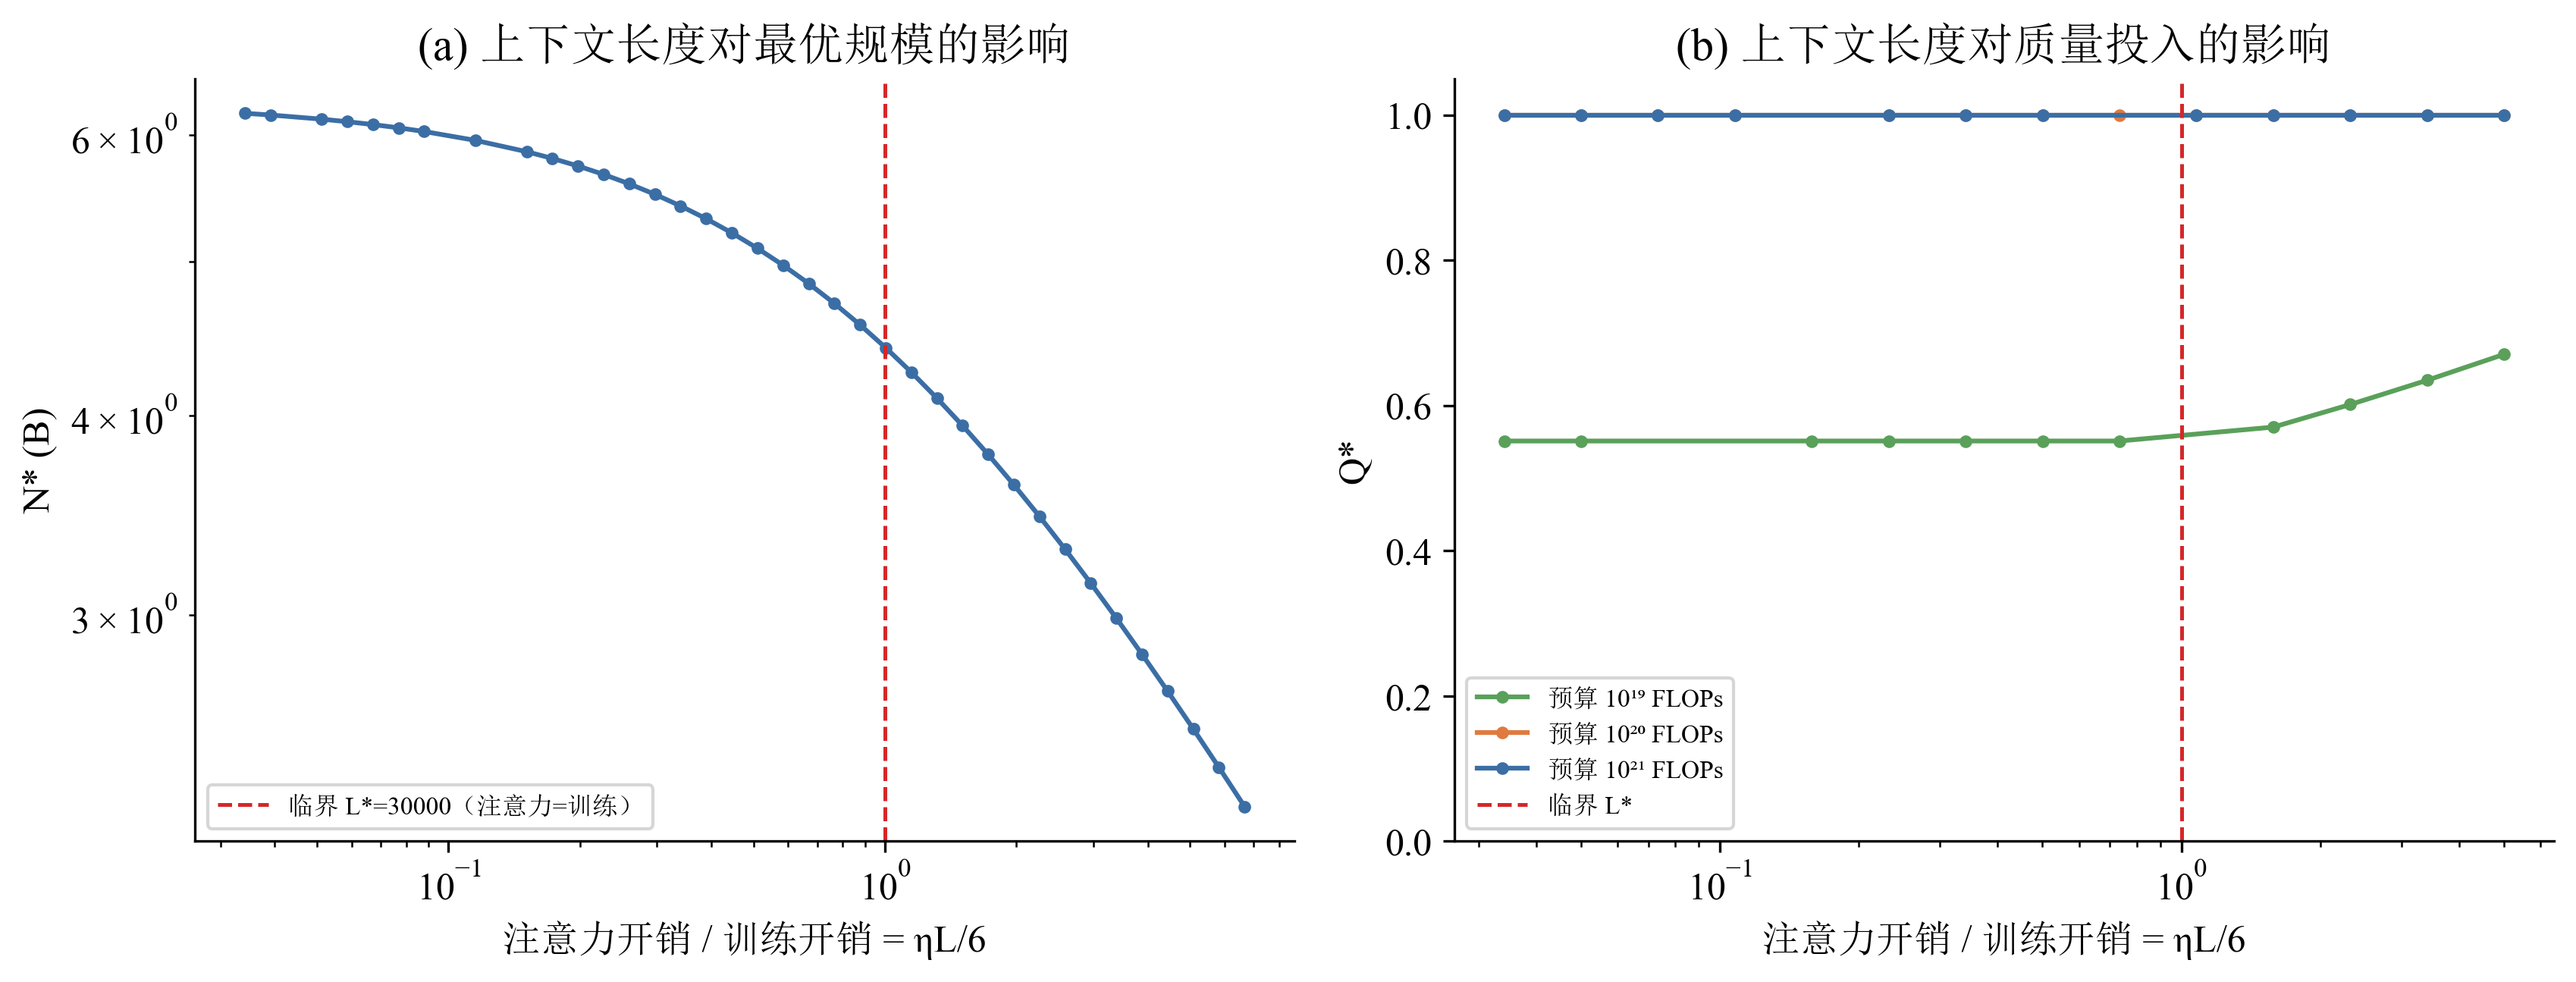
\includegraphics[width=0.92\textwidth]{求解/问题三/图片/图3_上下文长度敏感性.png}
  \caption{上下文长度敏感性（左：注意力开销对最优规模的影响；右：对质量投入的影响）}
  \label{fig:p3_ctx}
\end{figure}

由表\ref{tab:p3_ctx}可知，C7 的五个可行取值恰好跨越临界值 $L_{\text{crit}}=30{,}000$：$8{,}192$ tokens 时注意力开销仅为训练开销的 $0.273$ 倍，而 $32{,}768$ tokens 时已达 $1.092$ 倍、超过临界点。随上下文长度增长，注意力开销占比由 $5.7\%$ 升至 $77.3\%$，最优参数量被压缩 $2.25$ 倍、最优数据量被压缩 $2.10$ 倍，最优损失上升 $0.128$（约 $6.0\%$）。这一结论量化了“长上下文与规模投入存在算力竞争”的直觉：由于 $N^*\propto C^{\beta/(\alpha+\beta)}$，当基础训练单价被放大 $1+\lambda$ 倍时，可用于规模的等效预算按 $(1+\lambda)^{-\beta/(\alpha+\beta)}$ 缩减。需要说明的是，在 $C=10^{22}$ 这一预算档，即使 $L_{\text{ctx}}=131{,}072$，最优质量仍达上界 $1.000$，即长上下文的挤压主要体现在规模而非质量上——这与表\ref{tab:p3_shift}所示“中高预算下质量已饱和”的判断一致。

一个容易被直觉忽略的现象是：在**低预算档**，注意力开销上升反而使最优质量**提高**（图\ref{fig:p3_ctx}(b) 中 $C=10^{19}$ 曲线在 $L_{\text{ctx}}$ 由 $1{,}024$ 增至 $150{,}000$、注意力开销倍数由 $0.03$ 增至 $5.0$ 时，$Q^{*}$ 由 $0.551$（=基线，不投资质量）升至 $0.670$）。原因是本模型严格保留了赛题给定的“质量成本与训练 token 数成正比”结构 $C_Q=D[g(Q)-g(Q_0)]_+$：长上下文挤压了可负担的数据量 $D$，而 $D$ 越小，把整份语料提升到质量 $Q$ 的总开销越低，于是质量投入的相对价格下降、最优质量上移。这提示在真实训练中，长上下文与数据质量投入并非简单互斥，而是通过数据规模这一中间变量发生耦合——若采用“质量成本与数据量无关”的简化假设，这一耦合将被完全抹掉。

\textbf{4.领域配比的算力等价效果}

将问题一的推荐配比（$M=-0.1988$）与参考配比（$M=0$）在 $C=10^{22}$ FLOPs 下对比：两种情形的最优 $(N^{*},D^{*},Q^{*})$ 完全相同，但最优损失由 $2.1450$ 降至 $1.9462$。进一步用二分法求“参考配比达到同一损失所需的预算”，得 $C\approx3.05\times10^{23}$ FLOPs，即**领域配比优化的效果相当于约 $30$ 倍的算力扩张**。这为“调整领域配比虽不增加算力总开销，却会显著改变算力的使用效果”提供了定量证据。需说明的是，$M(\bm p)$ 是损失水平上的固定平移、与算力无关，因此换算为算力收益时会被损失的算力弹性放大，该倍数宜作量级参考而非精确比值。

综合以上结果，本节完成了问题三的求解：严格按赛题公式建立了含基础训练、质量提升与长文本注意力的成本模型，解析给出临界上下文长度 $L_{\text{crit}}=30{,}000$ tokens，求得三档预算下的最优资源配置，并以“质量投入启动边界 $1.78\times10^{19}$”与“质量接近饱和边界 $7.08\times10^{19}$”两个门槛识别出\textbf{基线质量期 $\to$ 质量提升期 $\to$ 质量饱和期}的三段式结构性转移。
